% !TeX program = xelatex
\documentclass[UTF8,a4paper,12pt]{ctexart}

\usepackage{amsmath}
\usepackage{booktabs}
\usepackage{caption}
\usepackage{float}
\usepackage{geometry}
\usepackage{graphicx}
\usepackage{hyperref}
\usepackage{siunitx}

\geometry{left=2.4cm,right=2.4cm,top=2.5cm,bottom=2.5cm}
\graphicspath{{figures/}}
\hypersetup{colorlinks=true,linkcolor=black,urlcolor=blue}
\sisetup{detect-all}

\title{使用手机陀螺仪和磁力计检测姿态的对比实验分析}
\author{基于 phyphox 采集数据}
\date{\today}

\begin{document}
\maketitle

\begin{abstract}
本文使用 phyphox 采集手机陀螺仪和磁力计数据，围绕静态漂移、定角度旋转和回归原点三个实验比较二者对水平姿态方向的估计能力。结果表明：陀螺仪在短时间内角度积分连续、重复性好，实验 2 中五个静止角度的误差均小于 \SI{1}{\degree}；但静态实验中仍可测得约 \SI{-0.207}{\degree\per\minute} 的零偏漂移。磁力计不需要时间积分，静态航向标准差约为 \SI{2.10}{\degree}，但对环境磁场十分敏感，定角度实验中最大误差达到 \SI{24.06}{\degree}，回归原点实验中还出现了磁场模长峰值 \SI{1676.8}{\micro\tesla} 的强干扰。实验支持的结论是：陀螺仪适合短时平滑跟踪，磁力计适合提供绝对方向约束，但单独使用任一传感器都不稳健，实际系统应采用互补滤波或卡尔曼滤波进行融合。
\end{abstract}

\section{实验目的}

手机陀螺仪测量角速度，绕竖直轴的角速度 $\omega_z$ 经时间积分后可得到相对航向角；磁力计测量地磁场在手机坐标系中的分量，可由水平分量直接估计相对地磁方向。二者都能反映手机姿态方向，但误差来源不同：陀螺仪受零偏和积分累积误差影响，磁力计受环境磁场畸变影响。本实验的目标是用同一部手机采集三组数据，定量比较二者的漂移、定角度精度和回到起点后的残余误差。

\section{数据与处理方法}

三组数据均来自 \texttt{data/} 目录，每组包含 \texttt{Gyroscope.csv} 和 \texttt{Magnetometer.csv}。陀螺仪采样率约 \SI{470}{\hertz}，磁力计采样率约 \SI{100}{\hertz}。数据集基本信息见表~\ref{tab:metadata}。

\begin{table}[H]
\centering
\begin{tabular}{lrrrrr}
\toprule
实验 & 时长/s & 陀螺仪样本 & 陀螺仪/Hz & 磁力计样本 & 磁力计/Hz \\
\midrule
exp1 & 32.00 & 15035 & 470.0 & 3198 & 100.0 \\
exp2 & 33.59 & 15780 & 470.0 & 3357 & 100.0 \\
exp3 & 67.02 & 31492 & 470.0 & 6700 & 100.0 \\
\bottomrule
\end{tabular}

{\vspace{0.4em}\small 采集设备：Xiaomi 24129PN74C。\par}
\caption{数据集基本信息}
\label{tab:metadata}
\end{table}


陀螺仪角度采用梯形积分：
\begin{equation}
  \theta_g(t_i)=\sum_{k=1}^{i}\frac{(\omega_z(t_k)-b_z)+(\omega_z(t_{k-1})-b_z)}{2}
  (t_k-t_{k-1}),
\end{equation}
其中 $b_z$ 是由实验 1 静止段估计的陀螺仪零偏。磁力计航向角采用
\begin{equation}
  \theta_m=-\operatorname{atan2}(B_y,B_x).
\end{equation}
负号用于使磁力计角度方向与本数据中的陀螺仪 $z$ 轴正方向一致。由于本次数据没有使用加速度计进行倾角补偿，磁力计结果只作为相对水平航向的近似估计。

实验 2 的静止角度段由 $\lvert\omega_z\rvert$ 的 \SI{0.20}{\second} 滚动均值自动识别，阈值取 \SI{0.03}{\radian\per\second}，持续时间至少 \SI{0.50}{\second}；相邻间隔小于 \SI{0.80}{\second} 的静止段合并。为减小转动开始和结束瞬间的影响，每段只取中心 \SI{60}{\percent} 的数据计算平均角度和标准差。所有处理由 \texttt{src/analyze.py} 完成，生成的中间结果保存在 \texttt{report/processed/}。

\section{结果}

\subsection{实验 1：静态漂移}

手机平放静止约 \SI{32}{\second}。静态段中陀螺仪 $z$ 轴零偏为 \SI{-6.02e-5}{\radian\per\second}，折算漂移率为 \SI{-0.207}{\degree\per\minute}；未经校正的积分角度在 32 秒后偏移 \SI{-0.110}{\degree}。磁力计航向不发生积分漂移，但围绕均值抖动，标准差为 \SI{2.10}{\degree}。图~\ref{fig:exp1} 和表~\ref{tab:exp1} 显示了这一差异。

\begin{figure}[H]
  \centering
  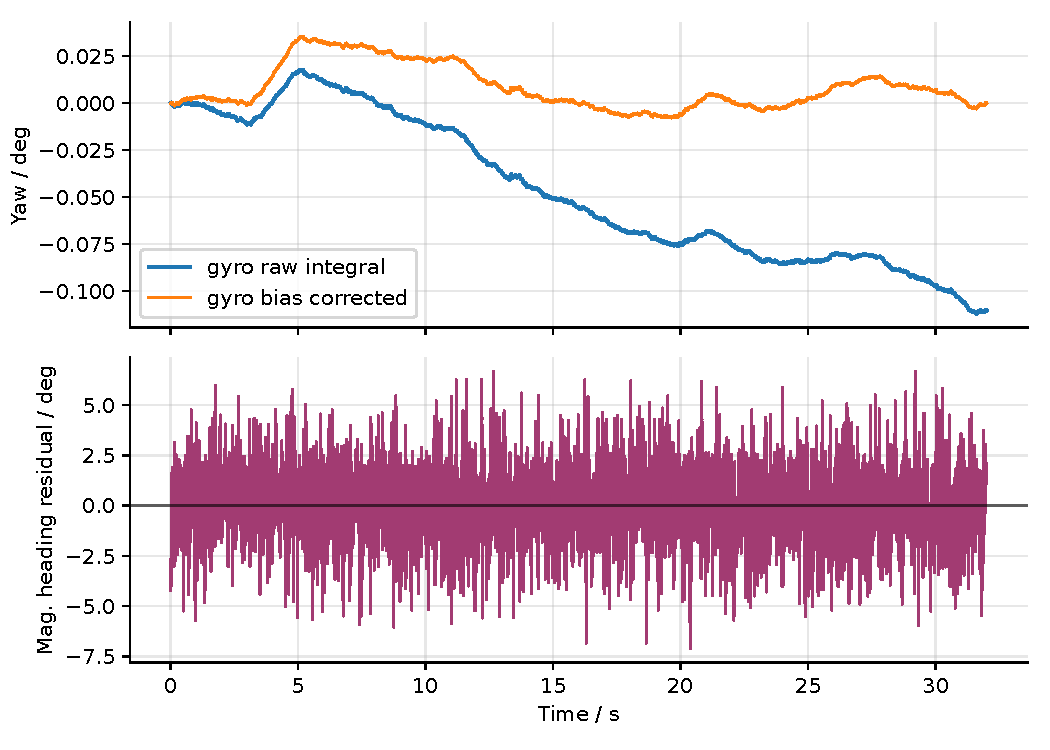
\includegraphics[width=0.92\linewidth]{exp1_static.pdf}
  \caption{实验 1 静止时的陀螺仪积分角和磁力计航向残差。陀螺仪未经校正时呈缓慢线性漂移；磁力计无累积趋势，但短时噪声更明显。}
  \label{fig:exp1}
\end{figure}

\begin{table}[H]
\centering
\begin{tabular}{lrl}
\toprule
指标 & 数值 & 单位 \\
\midrule
陀螺仪 $\omega_z$ 零偏 & -0.000060 & rad/s \\
陀螺仪等效漂移率 & -0.207 & $^\circ$/min \\
未校正积分终值 & -0.110 & $^\circ$ \\
零偏校正后积分终值 & 0.000 & $^\circ$ \\
磁力计航向标准差 & 2.102 & $^\circ$ \\
磁场模长均值 & 48.03 & $\mu$T \\
磁场模长标准差 & 0.82 & $\mu$T \\
\bottomrule
\end{tabular}
\caption{实验 1：静态漂移统计}
\label{tab:exp1}
\end{table}


\subsection{实验 2：定角度旋转}

实验 2 依次经过约 $0^\circ$、$90^\circ$、$180^\circ$、$270^\circ$、$360^\circ$ 五个静止姿态。经过实验 1 零偏校正后，陀螺仪积分角在各静止段的误差均小于 \SI{1}{\degree}，且静止段内标准差很小。磁力计在 $90^\circ$、$180^\circ$ 和 $270^\circ$ 位置出现明显系统偏差，其中 $180^\circ$ 位置偏差达到 \SI{24.06}{\degree}。这说明磁力计给出的是绝对方向信息，但该绝对方向会被局部磁场畸变拉偏。

\begin{figure}[H]
  \centering
  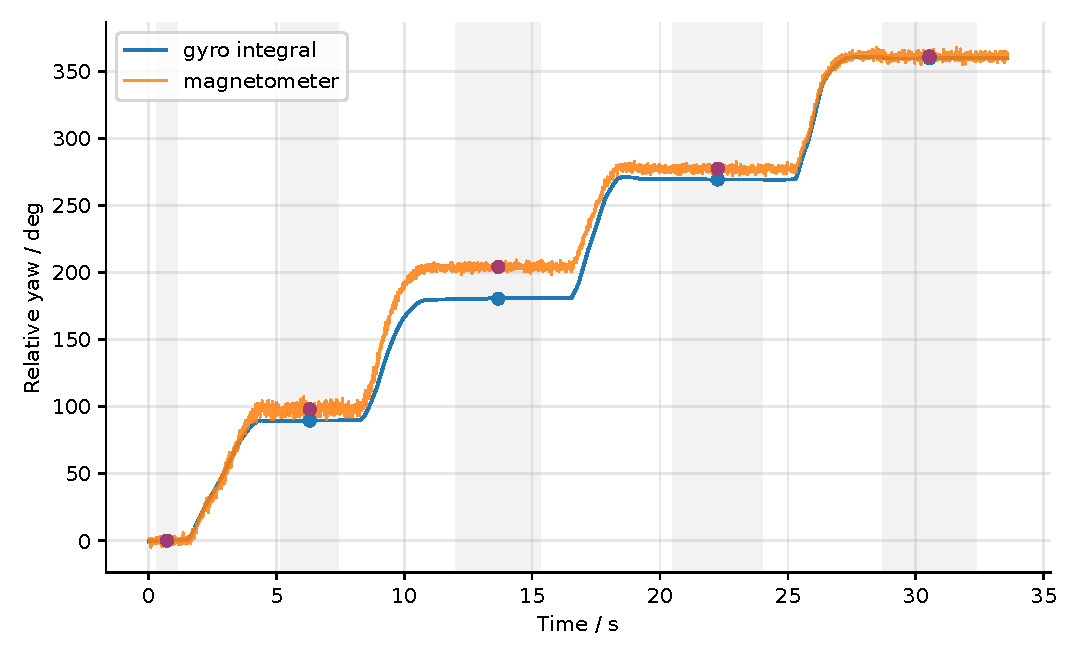
\includegraphics[width=0.92\linewidth]{exp2_step_response.pdf}
  \caption{实验 2 的相对航向角随时间变化。灰色区域为用于统计的静止段中心窗口。}
  \label{fig:exp2step}
\end{figure}

\begin{figure}[H]
  \centering
  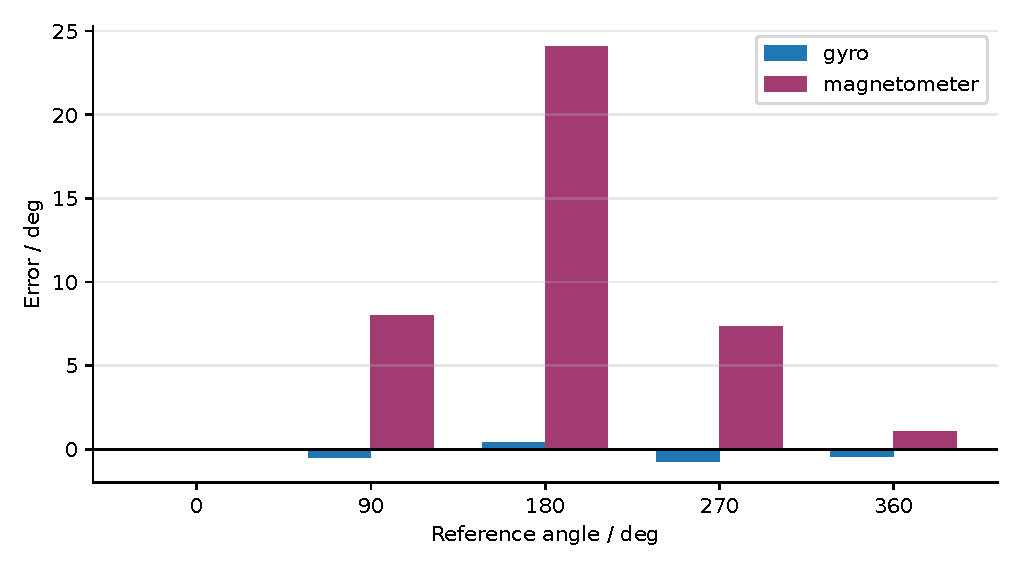
\includegraphics[width=0.86\linewidth]{exp2_errors.pdf}
  \caption{实验 2 各参考角下的角度误差。陀螺仪短时积分精度明显优于未校准磁力计。}
  \label{fig:exp2err}
\end{figure}

\begin{table}[H]
\centering
\begin{tabular}{rrrrrrr}
\toprule
参考角/$^\circ$ & 陀螺仪/$^\circ$ & 误差/$^\circ$ & 稳定段$\sigma$ & 磁力计/$^\circ$ & 误差/$^\circ$ & 稳定段$\sigma$ \\
\midrule
0 & 0.00 & +0.00 & 0.00 & 0.00 & +0.00 & 1.71 \\
90 & 89.48 & -0.52 & 0.02 & 98.01 & +8.01 & 3.29 \\
180 & 180.42 & +0.42 & 0.29 & 204.06 & +24.06 & 1.81 \\
270 & 269.25 & -0.75 & 0.07 & 277.34 & +7.34 & 1.74 \\
360 & 359.58 & -0.42 & 0.12 & 361.05 & +1.05 & 2.02 \\
\bottomrule
\end{tabular}
\caption{实验 2：定角度旋转结果}
\label{tab:exp2}
\end{table}


\subsection{实验 3：回归原点}

实验 3 持续约 \SI{67}{\second}，绕 $z$ 轴转动后回到起始朝向。陀螺仪积分总角度约为 \SI{1080.44}{\degree}，即接近 3 圈；扣除最近的整圈数后，回零残余为 \SI{0.44}{\degree}。磁力计起终窗口的航向差为 \SI{11.07}{\degree}，没有表现出理想情况下“直接回到初始读数”的特性。图~\ref{fig:exp3} 下半部分显示，在约 \SI{42.08}{\second} 处磁场模长峰值达到 \SI{1676.8}{\micro\tesla}，远高于正常地磁量级，说明实验过程中存在强磁干扰；这也是磁力计残余误差偏大的主要原因。

\begin{figure}[H]
  \centering
  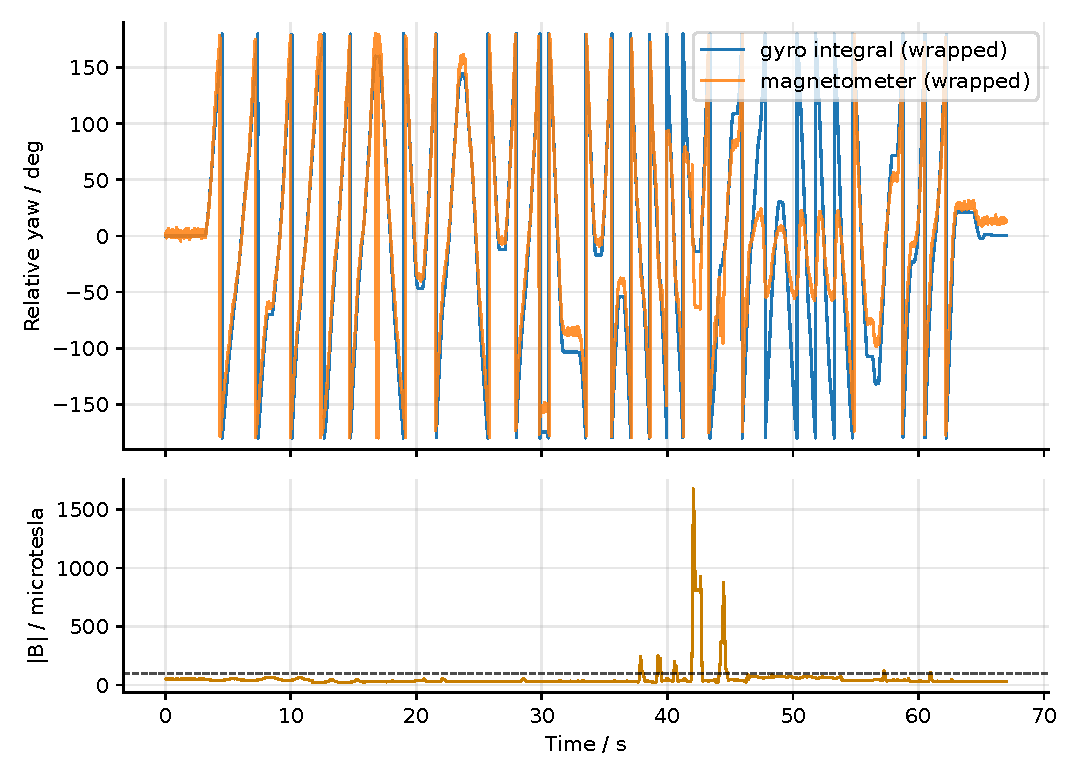
\includegraphics[width=0.92\linewidth]{exp3_return.pdf}
  \caption{实验 3 的回归原点结果。上图为包裹到 $[-180^\circ,180^\circ]$ 的相对航向角，下图为磁场模长。虚线为 \SI{100}{\micro\tesla} 的强干扰参考阈值。}
  \label{fig:exp3}
\end{figure}

\begin{table}[H]
\centering
\begin{tabular}{lrl}
\toprule
指标 & 数值 & 单位 \\
\midrule
陀螺仪积分总角度 & 1080.44 & $^\circ$ \\
最近整圈数 & 3 & 圈 \\
陀螺仪回零残余 & 0.44 & $^\circ$ \\
磁力计起终航向差 & 11.07 & $^\circ$ \\
磁场模长均值 & 55.08 & $\mu$T \\
磁场模长最大值 & 1676.8 & $\mu$T \\
强干扰样本占比 & 3.66 & \% \\
\bottomrule
\end{tabular}
\caption{实验 3：回归原点结果}
\label{tab:exp3}
\end{table}


\section{讨论}

从三组实验可以分离出两类误差特性。陀螺仪的优势是短时间内角速度测量连续、动态响应好，积分曲线平滑；在本次约半分钟的定角度实验中，只要用静止段估计并扣除零偏，就可以达到约 1 度以内的相对角度误差。其弱点是积分会把零偏和低频误差累积为角度漂移，静止时测得的 \SI{-0.207}{\degree\per\minute} 漂移率虽然不大，但在更长时间、温度变化或零偏变化时会继续累积。

磁力计的优势是它不依赖时间积分，因此理论上不会出现陀螺仪那种随时间线性累积的漂移；静止实验中它只是围绕均值抖动。然而磁力计测到的是手机附近的总磁场，不只包含地磁场，也包含桌面、电脑、金属物体、电流和磁性器件造成的硬铁、软铁干扰。本数据中实验 2 的 $180^\circ$ 位置误差达到 \SI{24.06}{\degree}，实验 3 的磁场模长峰值更达到 \SI{1676.8}{\micro\tesla}，这些都表明未经磁校准的磁力计不能稳定承担高精度姿态判断。

因此，本实验并不能得出“某一个传感器绝对更好”的结论。更合理的工程结论是：陀螺仪负责短时动态和高频变化，磁力计负责长期绝对方向约束；通过互补滤波或卡尔曼滤波，让磁力计慢速修正陀螺仪漂移，同时避免磁力计短时干扰直接污染姿态角，才是更稳健的方案。

\section{结论}

在本次 phyphox 数据中，陀螺仪静态漂移率约为 \SI{-0.207}{\degree\per\minute}，但经过零偏校正后，定角度旋转实验的误差控制在 \SI{1}{\degree} 以内；磁力计静态航向标准差约为 \SI{2.10}{\degree}，但在局部磁场干扰下定角度误差可达 \SI{24.06}{\degree}，回归原点残余也达到 \SI{11.07}{\degree}。陀螺仪和磁力计分别体现了“短时稳定但长期漂移”和“无积分漂移但环境敏感”的典型特征。实际室内定位或姿态估计中，应结合二者而不是单独依赖其中之一。

\end{document}
